%=========================================================================
% (c) Michal Bidlo, Bohuslav Křena, 2008

% Zajimavy blog
% http://brendangregg.com/


\chapter{Introduction}
\label{Introduction}
Good application performance is one of the main goals during the software development. But what makes software performance so important? Software reliability has to be guaranteed by the owner, but with undesirable performance there could be a lot of issues. Thus can badly influence software behavior. And this can cause a significant outflow of the consumers, and even brand destruction, financial damage, or loss of trust. These few reasons should be enough to do a proper performance testing before every software release, especially for large projects where industries guarantee certain level of software behavior and they would not be able to assure it with insufficient performance testing. Great emphasis on software performance is, in particular, in space programs, medical facilities, army systems, or energy distribution systems. In these fields it is necessary to ensure proper application behavior for a long time under high load and without any unexpected behavior such as high response time, frequent delays, or timeouts, because every failure is paid dearly. 

Nowadays every developer should try to use well established frameworks which can make theirs work easier. Frameworks handle complex underlying issues such as security, performance, and code clarity. This way developers can invest more time in the actual functionality and meet the application requirements, since frameworks are usually optimized for one particular job. In the past every developer had to spent significant portion of development time tuning performance which led to spending more time and money for software development. But not everyone has enough knowledge of performance testing and this makes performance analysis and optimization even more difficult. This leads to a need for specialized performance tools which can provide more sophisticated information, however, actually useful tools are usually proprietary and/or too expensive.

A~very important part of the performance analysis is the right choice of \emph{key performance indicators} (KPIs) \cite{Molyneaux:TAoAPT} and effective interpretation of the results. The right choice of KPIs allows faster detection of performance problems and help developers with fixes and meeting the \emph{performance standards} \cite{Molyneaux:TAoAPT} set up by application owner or customer in time before the release. 

In general an application performance is important. However, smooth network application or hardware performance became much more demanded nowadays, since most of the communication is via the Internet.  Obviously when you make a payment in your internet banking you definitely want to have a stable connection to your bank's website without any delay. Network stability is significantly influenced by network components like routers and switches and hence their performance should be under utmost case. We refer to network performance testing as measurement of network service quality which is directly influenced by \emph{bandwidth, throughput, latency}, etc. 

For performance testing of particular network messaging system developed by \emph{Red Hat Inc.} there is an existing solution\,---Messaging Performance Tool (MPT) \cite{ORPISKE:MSGPT}. MPT is specialized for the performance testing of \emph{Message Broker} (Broker) \cite{RH:Broker}\,---\,network application level software cooperating with \emph{Qpid-dispatch service} \cite{RH:Interconnect} in the network as the message distributor. Unfortunately, the current version of MPT does not support performance testing of enough component like the Router component, Qpid-dispatch. In this work we will focus on this particular short coming and develop a worthy solution allowing proper performance testing of the Qpid-dispatch service.

This thesis is structured as follows. First, we define fundamentals of performance testing in Chapter \ref{Fundamentals of Software Performance Testing}. The rest of the thesis focuses on performance testing and analysis of Qpid-dispatch, an application level router designed by Red Hat Inc. Qpid-dispatch performance testing is based on MPT described in Chapter \ref{Messaging Performance Tool}. Description includes \emph{measurement process} and \emph{measured data description and evaluation}.The main goal of the thesis is to analyze MPT and design module for the Qpid-dispatch performance testing as described in Chapter \ref{Analysis and Design} together with used protocols and \emph{Automatic Topology Generator} for semi-automated network generation and deployment. Used technologies, tools and  implementation processes of each component are described in Chapter \ref{Implementation}. The most important part of the thesis is Chapter \ref{Experimental Evaluation}, containing the data gathering  from routers located in different types of topology, data evaluation and representation which leads to conclusion about performance of Qpid-dispatch. Finally, Chapter \ref{Conclusion} summarizes the thesis and proposes ideas for future use of developed tool.

% https://www.seguetech.com/what-is-software-performance-testing/

\chapter{Fundamentals of Software Performance Testing}
\label{Fundamentals of Software Performance Testing}
Usual goal of performance testing is to ensure that the application runs reasonably fast enough to keep the attention of users, even with unexpected amount of clients using the application at the same time. But why is it so important to have the application optimized for the best speed? Simply, when your application have slow response, long load time or bad scalability, the first website which user will visit afterwards will be web of your competitor. That is the reason why speed is currently one of the most significant performance factor of common performance problems. This chapter summarizes the fundamentals of performance testing which includes common performance processes, issues, and metrics, based on knowledge available in \cite{Molyneaux:TAoAPT, Kurkova:Thesis:2017, DIN:PHD, ISTQB}.


\section{Performance Testing Process}
\label{Performance Testing Process}
The main goal of the performance testing is to ensure the following application attributes \cite{GAO:MEASURING}:

\begin{description}
	\setlength\itemsep{0em}
	\item \textbf{Reliability and Stability}\,---\,the ability of software to perform its functions in system environment under some system load for acceptable \footnote{During software development there is a document with Software Requirements Specification which specifies software metrics, including performance.} period of time,
	\item \textbf{Scalability}\,---\,the ability of software to behave properly under various types of system load and handle increasing amount of workload (such as network traffic, server load, data transfer, etc.) which need new hardware for cluster expand,
	\item \textbf{Processing time and Speed}\,---\,the ability of software to react quickly without low response time during any acceptable system load,
	\item \textbf{Availability}\,---\,the ability of software to make all of its functions available during any acceptable system load. The ability of software, deployed in cluster, to provide all functions during node crash is called High Availability.
\end{description}

Similarly to software development process, performance testing process consist of usual engineering steps ranging from requirements definition to data evaluation. These steps also includes design, implementation, and execution of performance tests with data collection. The graphical representation of the performance testing process is depicted in the Figure~\ref{fig:performace_testing_process}. 

\begin{figure}[H]
  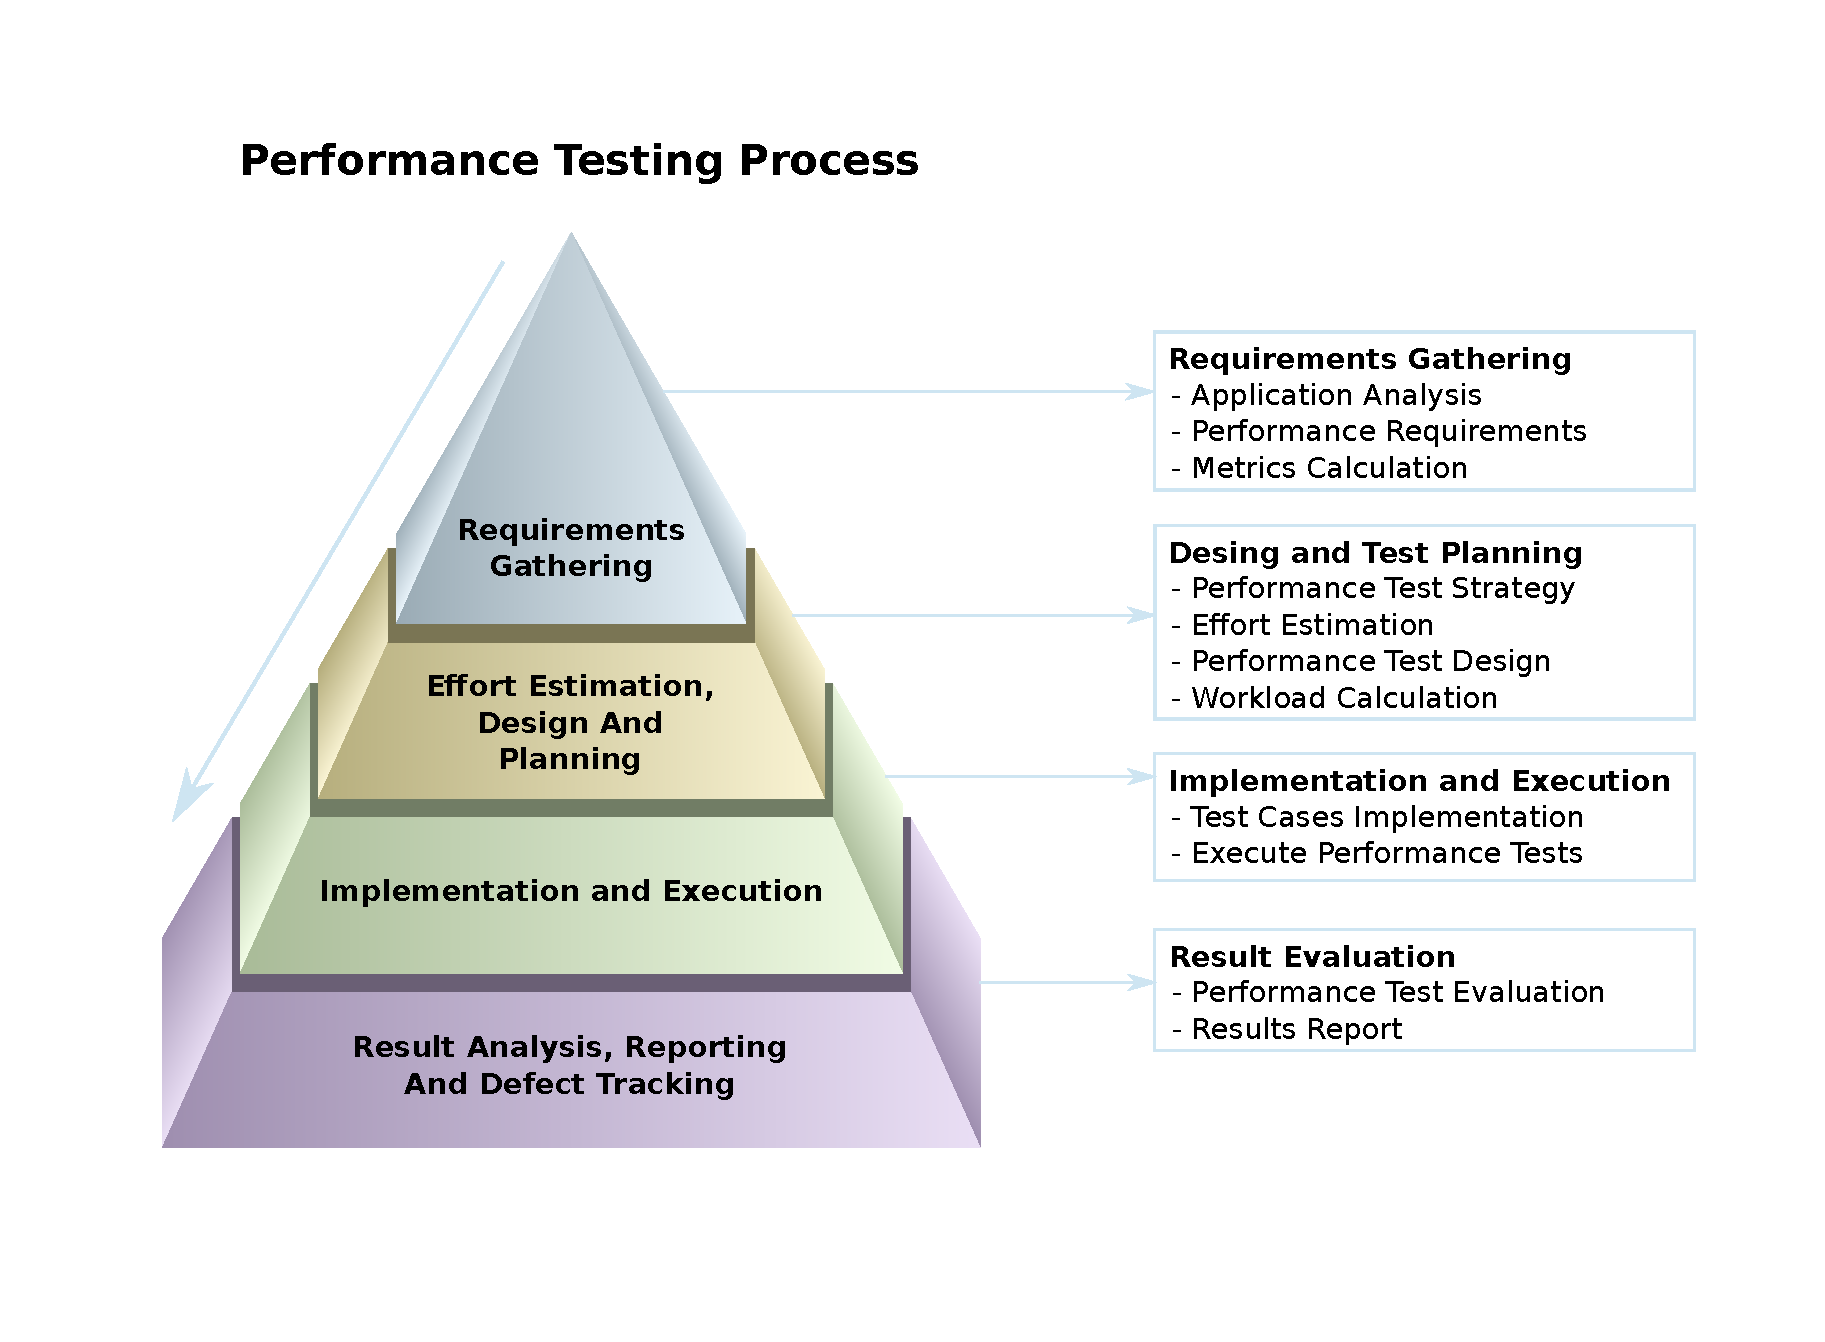
\includegraphics[width=16cm]{obrazky-figures/pyramid.pdf}
  \captionsetup{justification=centering}
  \caption{Performance Testing Process with the four most important parts and theirs individual steps based on \cite{Sharma:HP}.}
  \label{fig:performace_testing_process}
\end{figure}
In the Figure \ref{fig:performace_testing_process} you can see scheme of performance testing process where each level represent time for each step. Lower level refer to more time spend on that step.

The first step of performance testing process is the selection of \emph{performance requirements} for the application. In this step, testing engineer has to analyze \emph{software under test - SUT}, suitable performance metrics, that will model the application performance, and set performance requirements usually with customer and project manager. The result should include answers to questions such as:

\begin{itemize}
	\setlength\itemsep{0em}
	\item How many end users will the application need to handle at release, after 6 months or in 1 year ?
	\item Where will these users be physically located, and how will they connect to the application?
	\item How many end users will be concurrently connected in average at release, after 6 months and 1 year?
\end{itemize}

Based on answer to these studies, the engineer should be able to select important key performance indicators for performance test cases. Some of these indicators may be \emph{response time}, \emph{stability}, \emph{scalability}, or \emph{speed}. However, there is huge amount of possible indicators so it is necessary to properly analyze the whole application and also take into consideration another needs like an error rate, system resources, etc.  Result of this phase should be a binding document with all performance requirements to be tested and, in case of detected performance degradation, such defect must be fixed with reference to this document.

The next step is to define the \emph{performance testing strategy}, corresponding to planning and design. It is extremely important to allocate enough time for SUT testing effectively, because, as it was mentioned in Chapter \ref{Introduction}, performance testing is not an easy task and detecting all of the possible issues of tested components is very time consuming process. Every plan should take into account the following considerations:

\begin{description}
	\setlength\itemsep{0em}
	\item \textbf{Prepare the test environment}\,---\,this step include choosing right hardware for testing, then installing the necessary software for running load injectors, tested components, etc., and other equipment depend on application purpose such as routers, switchers, mobile devices, etc.
	\item \textbf{Provide sufficient workload injectors}\,---\,preparing the workload injector may take few days; we usually requires a few workstations or servers to simulate real traffic.
	\item \textbf{Identify and implement use cases}\,---\,this include identification of important parts of the system which may have an impact on performance; time needed for each use case may be different because some use cases can be simple such as navigating to a web application home page, but some may be complex such as filtering specific communication.
	\item \textbf{Instrument the test environment}\,---\,install and configure the monitoring software on the test environment.
	\item \textbf{Deal with detected problems}\,---\,test can detect significant performance issues, but their investigation and fix may take a long time. After fix the retest of issue is needed.
\end{description}

While this process seems trivial, the opposite is true, in especially in case of network applications. Most of performance issues manifest at big workloads or high number of users, e.g. when million users are sending requests to the network device at the same time it could lead to an unacceptable device crash. Workload injectors are designated to simulate real user activity, and allows automatic analysis of performance behavior for tested application or device. Depending on the used technology, there can be a limit on the number of virtual users that can be generated by a single injector. These automated workload injectors are necessary for effective performance testing.

After describing the plan we implement and execute proposed test cases. Environment and workload injectors are ready for execution, so last step before the testing itself is the implementation of tests. Thanks to the careful planing, engineers should have enough time to implement test cases with reference to proposed design. 

Final step of performance testing process is results evaluation. Output of this step is usually technical report with all selected performance key indicators, used workload and collected data for each test case. Then follows the data evaluation with thorough analysis of degradation localization. Additionally, the report usually contains syntactical graphs which display performance metrics along the duration of test execution.

\section{Performance Issues}
\label{Performance Issues}
\emph{Performance issue} is a common label for an unexpected application or device behavior which affects its performance. Usually, those issues are hard to detect because they manifest only under certain circumstances such as high load or long application run time. In the network applications there are several particular issues that are more frequently occurring  than others. In following, I will describe selected issues in more detail.

\subsection*{Performance Degradation}
\label{Performance Degradation}
Unclean code usually leads to inefficient algorithms, application deadlocks, or memory leaks, which all can eventually cause the performance degradation. The problem is that these issues are usually detected only during the long run time of application or inability of an application to handle high load. For this kind of issues there is a performance testing method called \emph{soak testing} \cite{BUCH:4TYPES, Manzor:APTB} which is described in Section \ref{Endurance Testing}. Soak test is intended to identify problems that may appear only after long period of application run-time\footnotemark, hence its necessary to run this type of tests during application development. The network applications are usually need to be available for 24 hours per day. The duration of a soak test should have some correlation to the operational mode of the system under test. Following scenarios may represent performance issues detectable by soak tests:

\begin{itemize}
	\setlength\itemsep{0em}
	\item a constant degradation in response time, when the system is run over the time,
	\item any degradation in system resources that are not apparent during short runs but will surface during long run time such as free disk space, or memory consumption
	\item a periodical process that may affect the performance of the system, but can be detected only during long run time as backup process, exporting of data to a 3rd party system, etc.,
	\item development of new features for already exists components.
\end{itemize}

\footnotetext{Soak Test - refer to HW testing method during which engineers soak device into water and check for bubble leaks.}

\subsection*{Response Time}
\label{Response Time 1}
Response time is how long it takes system to accept, evaluate, and respond to the user for his request e.g. HTTP request for particular website. Different actions and requests can have significantly different response time and with that provide different load on the system. For example retrieving document from web-server by its ID is considerably faster than searching for the same document by keywords. Response time is mostly measured during the \emph{load test} \cite{Manzor:APTB} of the application. Well designed test should consider different types of load on the system, various kind of requests, and different number of connected end-users at the same time. For user based systems we usually consider 3 threshold for the response time values: 

\begin{description}
	\setlength\itemsep{0em}
	\item \textbf{0.1 second}\,---\,this represent an ideal response time for the application, because user feels that system is reacting instantly and does not notice any interruptions.
	\item \textbf{1 second}\,---\,this is the highest acceptable response time when user still does not feel any interruptions, but can feel a little delay; this still represent no bad impact on the user experience.
	\item \textbf{10 second}\,---\,this is the limit after which response time become unacceptable and user will probably stop using your application.
\end{description}

However response time limits for non-human interactive system are more strict. They could acquire values in milliseconds or less.

\todo{Prvni iterace}

\subsection*{Traffic Spikes}
As \emph{traffic spike} \cite{Kurkova:Thesis:2017, AMC:SPIKES} we can understand the sudden degradation of one of the performance metrics such as \emph{throughput, bandwidth, error rate, response time} but also resource usage such as \emph{memory usage, disk space, etc.} during the network traffic. In real network, spikes are result of high workload, e.g. caused by higher amount of users trying to concurrently use the service over the network. For example we can experience sudden traffic spike in response time after publishing new popular viral context on video servers, start of sales events, reservation of limited amount of tickets or subject registration at university.

Traffic spikes can lead to inappropriate system behavior such as \emph{long response time}, \emph{bad throughput} and \emph{limited concurrency}. To prevent the impact of traffic spikes on system performance, it is  necessary to do sophisticated infrastructure monitoring and network load analysis, in order to distinguish between normal traffic and attack on the system. Suitable method for testing of spikes is called \emph{stress testing} \cite{Manzor:APTB} and it is described in Section \ref{Types of Performance Testing} in more details. Network system should also be scalable, thus it should be able to redirect traffic to another node with same service in case of high load which can cause performance issues due inappropriate resource usage.

\begin{figure}[H]
  \centering
  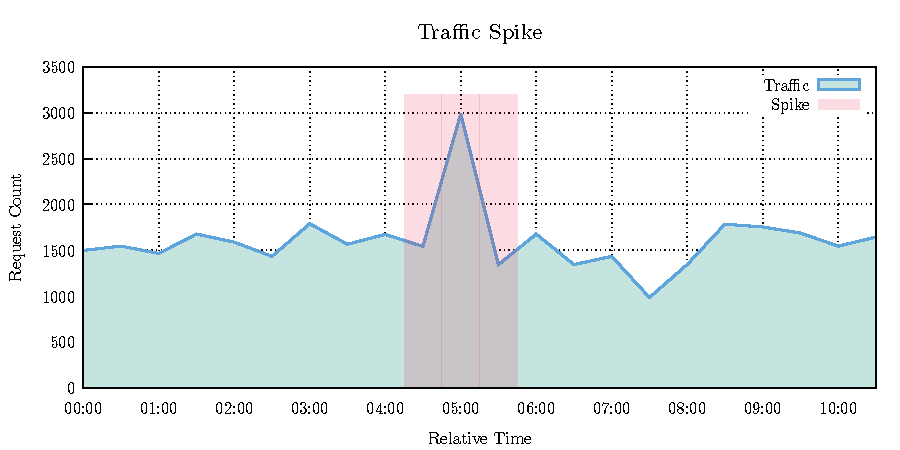
\includegraphics[width=14cm]{obrazky-figures/traffic_spike.pdf}
  \caption{The graph shows amount of concurrent sessions depending on time. During to network traffic monitoring the traffic spike occurring after 5 hours from test start.}
  \label{fig:spikes}
\end{figure}

\section{Types of Performance Testing}
\label{Types of Performance Testing}
% % http://www.wmrichards.com/high_performance_messaging.pdf 2017/10/18

For performance testing there are many types of suitable test methods. Which test you should use is determined by the nature of the system, testing requirements or how much time we have left for the performance testing. The following terms are generally well known and used in practice and each of them characterizes category or suite of the tests:
\begin{itemize}
	\item \textbf{Testing methods}\,---\,load testing, stress testing, endurance testing, \todo{scalability, volume, recovery}
	\item \textbf{Testing approaches}\,---\,smoke testing, regression testing, benchmark testing
\end{itemize}

Their description is based on knowledge available in \cite{TuPo:TESTS, BUCH:4TYPES, Molyneaux:TAoAPT, ISTQB}.

\subsection*{Load Testing}
Finding maximal load is a testing method which studies how the system behaves during different types of workload within acceptable time range. Basically it simulates the real-world load. During the load test we mainly focus on metric response time of the system for requests. Requests are generated by users or another systems communicating with the SUT. Main goal is to determine if the system can handle required workload according to performance requirements. Load test is designed to measure the response time of system transactions under normal or peak workload. When the response time of the system dramatically increases or becomes unstable, we conclude that system reached its maximum operating capacity. After successful testing, we should mark the workload requirements as fulfilling or analyze collected data and report issues to the developers. In the Figure \ref{fig:load_test} you can see the graph of load test showing workload of raising requests to the web server at the same time where the system response time does not exceed 3.5 seconds.

\begin{figure}[H]
  \centering
  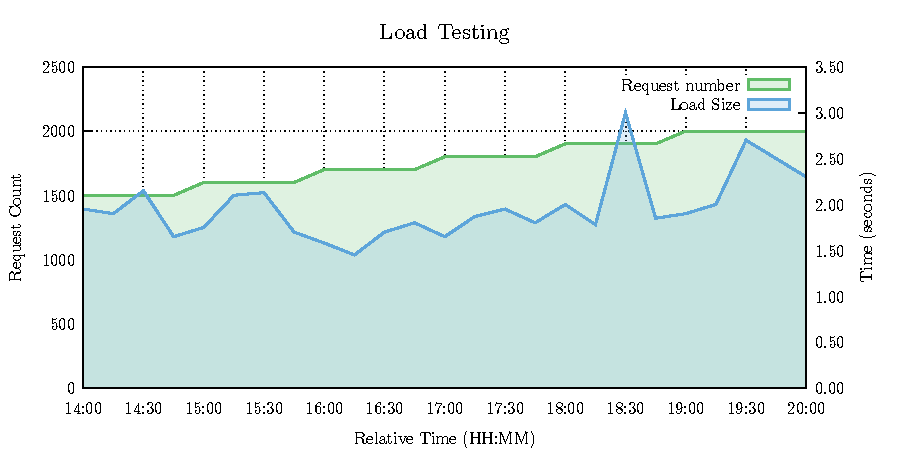
\includegraphics[width=15cm]{obrazky-figures/load_testing.pdf}
  \caption{Response time of the system during the load testing depended on by load size.}
  \label{fig:load_test}
\end{figure}

The following lists show common scenarios for load testing:
\begin{itemize}
	\setlength\itemsep{0em}
	\item The system interact with multiple users at same time.
	\item The system tracking communication and analyze it.
	\item Web services and information systems.
\end{itemize}
Typical system issues covered by load testing:
\begin{itemize}
	\setlength\itemsep{0em}
	\item Concurrent users connections can eventually result into slow response time or system crash.
	\item Network systems without redundancy connections can shutdown whole network under normal defined workload.
	\item Data availability during multiple session to data server.
	\item Connection rejection (timeout).
\end{itemize}

\subsection*{Stress Testing}
\label{Stress Testing}
Stress testing is the specific type of load testing, where we do not measure normal workload, but focus on unexpected workloads or traffic spikes. The main purpose is to study how the system behaves in extreme conditions such as enormous number of concurrent requests, using a server with much less memory or a weaker CPU, and analyze the system performance threshold. Its very useful to know performance threshold in order to know the difference between performance under normal workload and performance threshold. The following enumeration lists common stress test scenarios: 
\begin{itemize}
	\setlength\itemsep{0em}
	\item Monitor the system behavior with over maximum of users logged in at the same time.
	\item All user performing critical operations at the same time.
	\item All users accessing the same file at the same time.
	\item Hardware issues such as server in cluster down.
\end{itemize} 
Typical issues, which are covered by stress testing:
\begin{itemize}
	\setlength\itemsep{0em}
	\item Sudden performance degradation.
	\item System will recover after stress test (system is operational after test).
	\item System does not crash during stress test.
	\item All subsystems such as database, load balancer, etc. remains operational.
\end{itemize}

When engineers finish stress testing and found the limits of the system, they also can test the system recovery after crash during finding of the system limits.

In the Figure \ref{fig:stress_test} is recorded stress testing with raising load and response time. Everything is fine until the amount of requests exceed 3000 requests per second. With higher load there comes performance issues which leads to unexpected rise of the response time.

\begin{figure}[H]
  \centering
  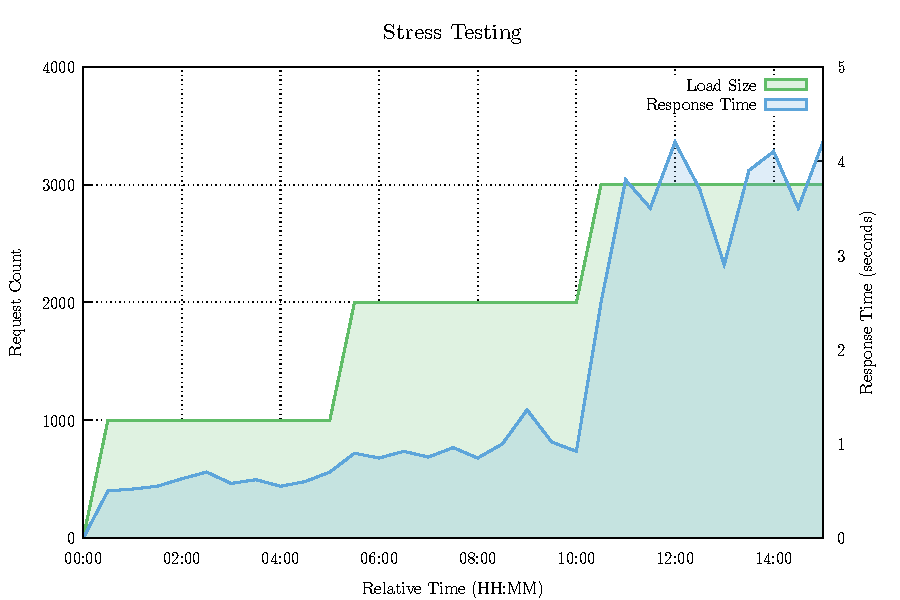
\includegraphics[width=15cm]{obrazky-figures/stress_testing.pdf}
  \caption{Stress testing diagram capturing dependency of response time on mount of requests.}
  \label{fig:stress_test}
\end{figure}

\subsection*{Endurance Testing}
\label{Endurance Testing}
Endurance, or stability/soak testing refer to the method, that tries to identify problems, that may appear only after the extended period of time e.g. The system could seems stable for one week, but after some longer period, problems such as memory leaks or not enough disk space can appear. Soak tests mainly focuses on measuring of memory as performance metric. The following are common issues found by soak test:
\begin{itemize}
	\setlength\itemsep{0em}
	\item Serious memory leaks that can eventually result into the system crash.
	\item Improperly closed database connections that could starve the system.
	\item Improperly closed connections between system layers that could stall any of the system modules.
	\item Step-wise degradation that could lead to high response time and the system becomes inefficient.
\end{itemize}
Typical scenarios for use soak testing:
\begin{itemize}
	\setlength\itemsep{0em}
	\item Developed system uses multiple database connections.
	\item There is a chance for inappropriately allocated memory, and memory free.
	\item Disk space limitation for store logs or other data.
\end{itemize}


This sort of test needs to use appropriate monitoring system to achieve high efficiency. Problems detected by soak tests are typically manifested by gradual system slowdown in response time or as a sudden lost of system availability.

\begin{figure}[H]
  \centering
  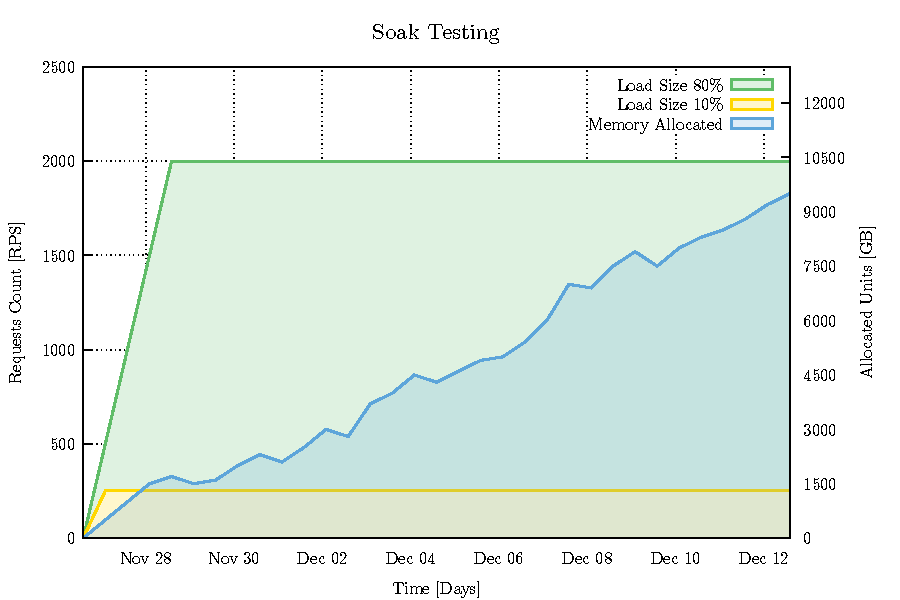
\includegraphics[width=15cm]{obrazky-figures/soak_testing.pdf}
  \caption{Soak testing with memory usage dependent on time.}
  \label{fig:soak_test}
\end{figure}

In the Figure \ref{fig:soak_test} you can see raising memory usage after period of time. The SUT can handle requests but as time goes by memory usage is to high that the SUT will crash. This may be caused by memory leak or an inappropriate algorithm use.

\subsection*{Smoke Testing}
Smoke testing approach is inspired by similar hardware technique, when engineers checks for presource of the smoke from the device after turning the power on. Basically, its similar for software, since main goal of smoke test is to test basic functionality of the system and guarantee that the system is ready for build. However, smoke tests are testing the functionality on a surface level, so it may not be enough for deep testing of basic system functions. When smoke tests fail, the system is tagged as unstable, because it cannot ensure its basic functionality and it is not tested anymore until the smoke test pass. Smoke test are designed to uncover obvious errors which saves time, money and effort of the engineers. These tests should be used with every new build, since new features could harm previous system functionality.
The following lists show common scenarios for smoke testing:
\begin{itemize}
	\setlength\itemsep{0em}
	\item New system's build or version is ready for further testing or productilization.
\end{itemize}
Typical system issues covered by smoke testing testing:
\begin{itemize}
	\setlength\itemsep{0em}
	\item System without main functionality is useless, because test coverage of functionality is low.
	\item Main functionality can result into system crash.
\end{itemize} 


\subsection*{Regression Testing}
Whenever engineers develop new feature and want to update the previous build it has to pass the \emph{regression tests}\footnotemark \cite{STF:REGRESSION}. Regression tests are designed to test functionality of the latest build updated with new feature. The main objective is to determine, if new feature affects already functional parts of the system. This type of tests is very important, because engineers do not always realize, which parts of the system will be indirectly affected. During regression testing, new test cases are not created, but previous test cases are automatic re-executed and analyzed. 
Typical scenarios for regression testing:
\begin{itemize}
	\setlength\itemsep{0em}
	\item New feature of system is ready for use.
\end{itemize}
Common issues covered by regression testing:
\begin{itemize}
	\setlength\itemsep{0em}
	\item New feature could adversely affect already working components of the system.
\end{itemize}

\footnotetext{{\label{note1}Approach for test suits, where are used other methods like Load testing, Stress testing, etc.}}

\subsection*{Benchmark Testing}
\emph{Benchmark testing}\textsuperscript{\ref{note1}} \cite{Aho:Benchmarking} is approach, which collects performance data during the system run on different hardware machines. Collected data have significant value when we want smooth run of the system on an older hardware, hence we can discover performance issues under normal load. However, the system does not run smoothly on prepared hardware, only options is to run benchmark tests on different machines with different hardware and under different load.

\begin{itemize}
	\item Can identify minimal requirements for HW, metrics, etc.
	\item Can validate supported HW configuration.
\end{itemize}



\section{Performance Metrics}
\label{Performance Metrics}
% https://loadstorm.com/load-testing-metrics/ 2017/10/18

During the performance testing we can monitor a lot of metrics, which can have different importance based on the system's purpose. The following lists the most common metrics that are monitored during the performance testing of all applications, no matter of developing language. 

In the testing systems, performance metrics are collected during long process of collecting, analyzing and reporting information regarding performance of whole system or individual component. This process can be different for each metric, since each metric needs different type of the system analysis.


\subsection{Throughput}
Throughput is a metric, which refers to the number of requests per second that the system can handle. \emph{Network throughput} is the rate of successful message deliveries over a communication channel. Throughput is usually measured after a warm-up period of time after the commencement of traffic, because it takes a while for workload to stabilize. We need stabilized workload for proper throughput measurement, because initial values could negatively affect the measurement. Throughput is measured by load testing; suitable strategy for measuring throughput is to continuously raise the load until response takes longer that acceptable threshold.

\subsection{Response Time and Latency}
Response time as issue was already mentioned in Subsection \ref{Response Time 1}; response time as metric is consists of two parts which are \emph{latency} and \emph{service time}.

\subsubsection*{Service Time}
Service time is the time it takes system to evaluate and send response to user request. In particular, when user sends request for a web page to a server, it takes the server time to evaluate the request and send proper response back to the user, this is the service time. Measurement can be performed easily using stopwatch which starts at receive of request and stops after the response is send. Service time can be affected by any item which leads to a performance degradation as described in Subsection \ref{Performance Degradation}. 

\subsubsection*{Latency}
Second part of the response time is latency \cite{Broadwell:RPT, BHATT:PERF}, which represent a delay between sending the request on the client side and receiving it for evaluation on the server side. Hence latency is the common problem in the network systems such as data center, web server, etc., because request/response needs to travel over the physical medium between the client and the server. Client and server could be located on different continents, thus the message have to travel long distance and latency is increasing.  

\begin{figure}[H]
  \centering
  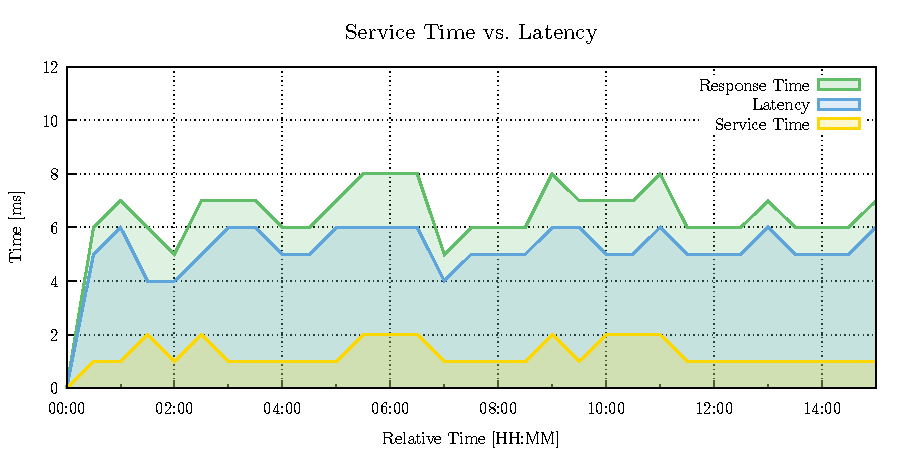
\includegraphics[width=15cm]{obrazky-figures/latency.pdf}
  \caption{Latency diagram with system's response time based on the date.}
  \label{fig:latency}
\end{figure}

\subsubsection*{Average and Percentile Response Time}
There are two common ways of measuring the response time \cite{Kopp:RPT}: Average (mean) response time is calculated as the sum of all measured times divided by the count of users requests. While this seems trivial, in many times, the average response time does not actually reflect the real response time of the system. How is that possible? In reality, most application have few heavy outliers such as very slow transactions. In the Figure \ref{fig:average_percentil_1} you can see few slow transactions which drag the average of the response time to the right. This naturally leads to an inaccurate specification of response time.


\begin{figure}[H]
  \centering
  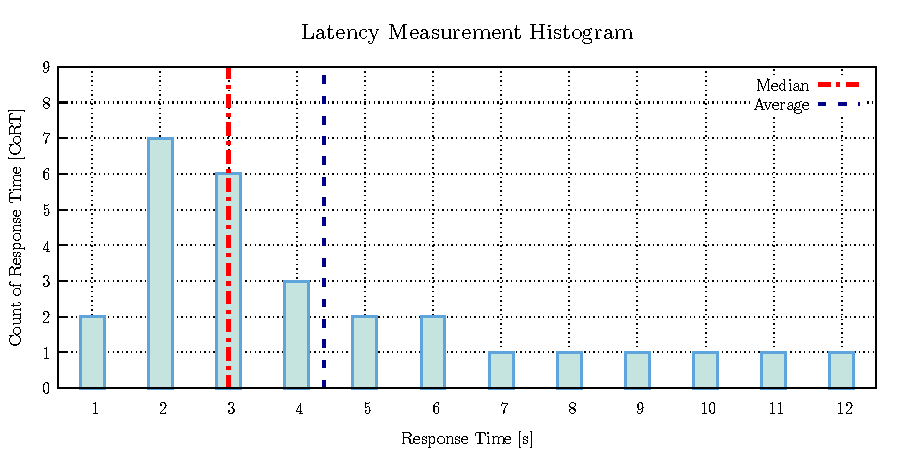
\includegraphics[width=15cm]{obrazky-figures/average_median_1.pdf}
  \caption{Transactions response time with calculated average and median of response time. Average represent  inaccurate response time in this case which is higher than real one.}
  \label{fig:average_percentil_1}
\end{figure}

The better solution how to determine the actual response time is Percentile. The percentile is statistic method, which cut measured ordered values into hundredths and then characterize the value below which a given percentage of measurements in a group of particular measurements falls. In the Figure \ref{fig:average_percentil_1} you can see the \emph{median} value, which reflects more realistic value of the system response time. Median value is same such as the 50th percentile. In this case, there is no problem, because user will expect slower response time than it has. 

\begin{figure}[H]
  \centering
  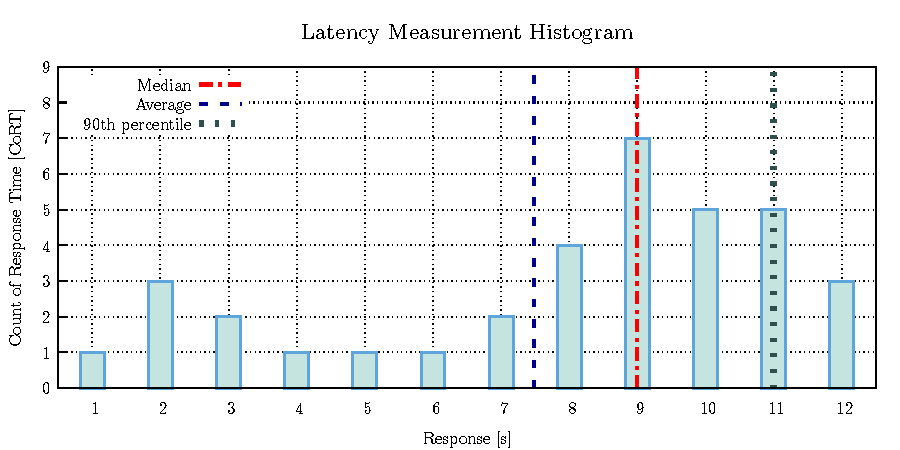
\includegraphics[width=15cm]{obrazky-figures/average_median_2.pdf}
  \caption{Transactions response time with calculated average and median of response time. Average represent  inaccurate response time. Average says, that STU is faster than is in reality.}
  \label{fig:average_percentil_2}
\end{figure}

The Figure \ref{fig:average_percentil_2} shows different situation. Average response time seems better than median, which reflects the expectation of faster system response time than it has. In real systems, we usually use values of the 90th percentile and the 99th percentile. 90th percentile mean, that there is only 10 \% transactions slower then marked response time. In the Figure \ref{fig:average_percentil_2}, a considerable percentage of transactions are very fast (first 50 percent), while the bulk of transactions are several times slower. Thus, calculated percentile gets more realistic values than average response time.

\subsection{Resource Usage}
Applications running at servers with long run-time competes over a limited amount of resource available for use. Thus makes resource usage another important metric, which needs to be monitored since not enough resources could shut down the whole system. Main resources for monitoring and utilization are:

\begin{description}
	\setlength\itemsep{0em}
	\item \textbf{CPU usage}\,---\,inappropriate usage of CPU could lead to performance degradation, because low priority processes may occupy CPU ahead of the higher priority processes. CPU usage is structuring into system usage and user usage. High system usage can cause problems or bottlenecks.
	\item \textbf{Memory usage}\,---\,full consumption of memory could cause performance degradation.
	\item \textbf{Disk space}\,---\,for example when using storage disk as a database, there should be preventive measures to backup the data and free up disk space.
	\item \textbf{Operating System limits}\,---\,system's memory, and CPU capabilities. 
\end{description}


\subsection{Error Rate}
Error Rate is a metric, which commonly occurs in the network systems, especially under high load. During the communication between client and server there could be error caused by another network device (router, switch, etc.) or signal disruption of the data during the transfer. The Error Rate is the mathematical calculation that produces a percentage of problem requests compared to all requests. In the ideal system, there should be zero network error present, however, in reality is in-feasible. This usually leads to a performance degradation and low throughput, because damaged data need to be resent.
Error rate is a significant metric because it tells engineers how many requests failed at a particular point in time of performance testing. This metric is more evident when you can see the percentage of problem strongly increasing, hence you can detect problem easily.


\todo{Druha iterace}

\chapter{Messaging Performance Tool}
\label{Messaging Performance Tool}
% https://github.com/orpiske/msg-perf-tool
Performance of \emph{Message-Oriented Middleware} (MOM) \cite{CURRY:MOM} is one of the most critical elements of quality assurence for enterprise integration system. There are multiple messaging components developed in Red Hat such as messaging clients, Message Broker, Message Router (Qpid-dispatch service) and stream-like message distributions tools. Since now, client has meaning of messaging client. \todo{Kafka - free to disclose? eric} 

A Message Broker is an example of MOM. Its purpose is receive, store and distribute messages, which are sent and received by clients. The performance capabilities of a Message Broker are important for its users, because being able to handle a large amount of transactions in a timely manner is an important characteristic of MOM. Users choose MOM for message distribution so they do not have to develop their own messaging distribution systems Another benefit of specialized MOM than own implementation is robustness and ensured performance. For example in automated systems, where components communicates with each other by command exchange. Amount of exchanged command is dependent on system size. We want to get systems results as soon as possible and for that is important to ensure smooth and quick message exchange.

\emph{The Maestro} \cite{ORPISKE:MSGPT} is a testing system designed especially for testing the performance of MOM. On the Figure \ref{fig:msg_perf_tool} you can see architecture of Maestro. The whole Maestro is deployed as a cluster system on several machines. A typical Maestro deployment consist of one node for Maestro Broker, one or more for Senders, one or more for Receivers and the SUT. The Maestro system consists of several components:

\begin{description}
	\setlength\itemsep{0em}
	\item \textbf{Maestro Broker}\,---\,any \emph{Message Queuing Telemetry Transport - MQTT\footnotemark}-capable broker with several topics. This component takes care about distribution of control messages between other cluster components such as Maestro Clients and MPT Back-end. 
	\item \textbf{Meastro Clients}\,---\,this component contains the client API as well as the test scripts for each test case. A sub-component called Reporter takes care of data reporting to the user, which means data visualization on the web.
	\item \textbf{MPT Back-end}\,---\,consists of sender part, receiver part and inspector part. Sender, and receiver ensure messaging sending to the SUT and receiving from it. Inspector monitoring workload over the SUT and reporting collected performance metrics to the testing cluster. Maestro currently has two back-ends:
	\begin{itemize}
		\item \textbf{Java}\,---\,using for JMS-based\footnotemark testing, including \emph{Advanced Message Queuing Protocol - AMQP} \cite{OASIS:AMQP}, OpenWire and Core protocols.
		\item \textbf{C}\,---\,using for AMQP and \emph{Streaming Text Oriented Messaging Protocol - STOMP}\footnotemark protocol testing.
	\end{itemize}
\end{description}

\begin{figure}[H]
  \centering
  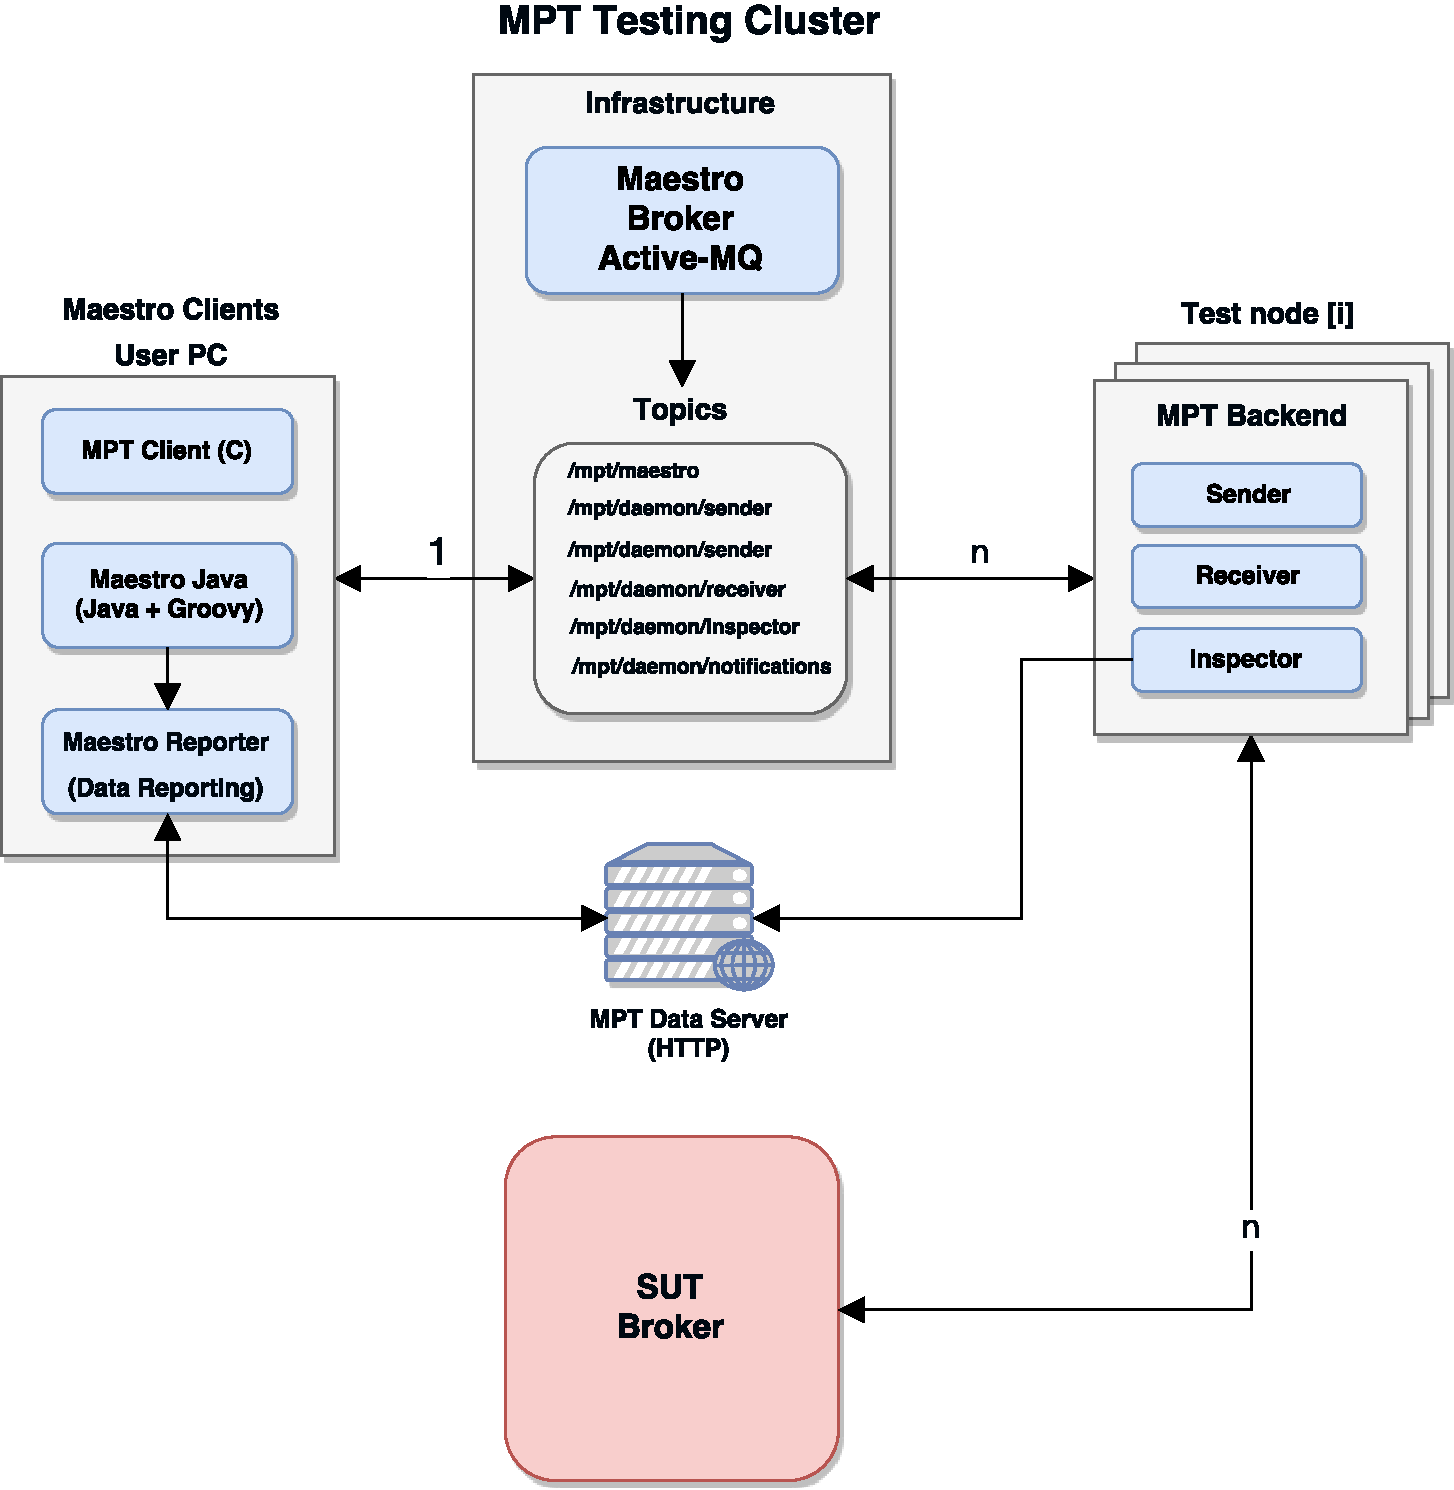
\includegraphics[width=15cm]{obrazky-figures/msg_perf_tool.pdf}
  \caption{Architecture of the Maestro.}
  \label{fig:msg_perf_tool}
\end{figure}

\footnotetext{MQTT - \url{http://mqtt.org/}}
\footnotetext{JMS - Java Message Service}
\footnotetext{STOMP - \url{https://stomp.github.io/}}

\section*{Test Case Scenario}
Configuration of each test case is specified by several options defined in Groovy \footnote{Object-oriented programming language for Java platform \url{http://groovy-lang.org/}} script. This script specify test behavior with following items:

\begin{itemize}
	\setlength\itemsep{0em}
	\item \textbf{message size}\,---\,message size in bytes,
	\item \textbf{number of connected clients}\,---\,count of senders and receivers connected to the SUT,
	\item \textbf{test duration (time or load)}\,---\,end condition of each test, could be specified by time or message count,
	\item \textbf{message rate}\,---\,the desired rate that the system should try to maintain (0 for unbounded).
\end{itemize}

The test script is also responsible for starting and stopping the test. We can also specify the test profile. Depending on the test profile, the script may also be responsible for increasing or decreasing the workload on the S.U.T during the test scenario. The load can be modified by increasing the target rate or the number of parallel connections. Multiple combinations of this options can create a lot of test cases with different load for the SUT. Every test will produce his own logs which are processed by the reporting sub-component on the client side and used for monitoring the metrics. Maestro Reporter produce data visualization, such as charts, from stored logs.

\section*{Measures Process}
\label{Measures Process}
Measures process starts after dynamic test generation with option passed from the test file. Sender or senders, depends on test file, will start sending messages to the SUT. Inspector starts monitoring the behavior of the SUT and write it to disk. For monitoring, Inspector uses the Broker management interface. That is a REST interface that exposes (via HTTP protocol) internal JVM \footnote{JVM - Java Virtual Machine} and Broker detailed information. That information would be normally available via JMX \footnote{JMX - Java Management Extensions}. Data collection by Inspector is simple and pretty straightforward:

\begin{itemize}
	\setlength\itemsep{0em}
	\item Inspector sent an HTTP request with the \emph{JavaScript Object Notation - JSON}\footnotemark content to the Broker REST interface.
	\item Broker evaluate the request and sent response to the Inspector.
	\item Inspector collect the response.
\end{itemize}
Errors occurred during the information collection may cause the test case fail.

However, there are two problem factors; the first is that inspector shouldn't influence performance of the SUT. Current method for information collecting working like the management interface call method with request for information and get response. During this call, the method usually involve locks to guarantee thread safety and exclusive access. However, calling this methods too often could cause Broker performance degradation. In order to reduce this risk, the inspector enforces a collection interval of 10 seconds and use only certain operations. That reduce the hits on management interface on 2 or 3 hits every 10 seconds.

The second is large size of the stored logs. This is mitigated by usage of the compression methods for reduction logs size. However, compressed logs can fill whole hard drive during long test-run, so old logs has to been erase at some point of time. The collected logs can be safely erased when the test is completed. The Maestro generates about 1\,Gb of uncompressed data per hour of testing.

%Inspector also monitor node with broker (CPU, memory size)?

%No. There's a new module being developed for that, which runs on top of Prometheus and monitors both the system and the test cluster: http://msg-qe-dev-01.tpb.lab.eng.brq.redhat.com:3000

\footnotetext{JSON - \url{https://www.json.org/}}

\section{Testing Metrics}
\label{Testing Metrics}
Which metrics are collected depending on the component. In the Table \ref{tab:maestro_metrics} we can see summary of the metrics, which are collected for each component.

\begin{table}[]
\centering
\begin{tabular}{|p{2.5cm}|p{3.5cm}|p{7cm}|}
\hline
\rowcolor[HTML]{C5E3DF} 
\multicolumn{1}{|c|}{\textbf{Component}} & \multicolumn{1}{c|}{\textbf{Metrics}} & \multicolumn{1}{c|}{\textbf{Description}}                       \\ \hline
\textbf{Sender}                          & Throughput                            & Throughput of the sender                                        \\ \hline
\textbf{Receiver}                        & Throughput                            & Throughput of the receiver                                      \\ \hline
\textbf{}                                & Latency                               & Time between send and receive message                           \\ \hline
\textbf{Broker}			                & JVM heap memory                       & maximum, minimum, and current Eden, Survivor, and Tenured space \\ \hline
                                         & JVM non-heap                          & PermGen or Metaspace                                            \\ \hline
                                         & Broker internals                      & Queue size and expiration count                                 \\ \hline
                                         & OS basic memory                       & Physical and swap memory usage                                  \\ \hline
                                         & OS resources                          & Count of file descriptors                                       \\ \hline
\end{tabular}
\caption{Maestro metrics summary.}
\label{tab:maestro_metrics}
\end{table}

 \todo{Dopsat}

\section{Collected Data and Their Evaluation}
\label{Collected Data and Their Evaluation}
As it was mentioned, data are collected by Inspector. 

\todo{Ask Otavio about inspector messages (format, data...)}



\section{Related Works}
\label{Related Works}
% popsat podobne "existujici" reseni (samozrejme, obcas neexistuje ;), ale verim, ze zde se neco najde). Nejlepsi je i se vuci tem "related tools" vymezit (jako napr. "The tool ... cannot be used because it does not support ...")

SpecJMS

\chapter{Analysis and Design}
\label{Analysis and Design}
MPT is generally designed for performance testing of Broker. However, with the service growth. the need for performance testing of Qpid-Dispatch comes. This Chapter is focused on two things: firstly, analyze Qpid-Dispatch service, describe its capabilities and methodology and secondly describe design of Topology generator and Qpid-Dispatch Performance Module for MPT.

\section{Qpid-Dispatch Router}
Qpid-Dispatch is a lightweight AMQP message router for building scalable available and performant messaging networks. With respect to ISO/OSI \footnotemark model, this router is an application layer program running as a normal user program or as a daemon. Key features of Qpid-Dispatch are:

\begin{itemize}
	\setlength\itemsep{0em}
	\item Connects clients and brokers into an internet-scale messaging network with uniform addressing.
	\item Supports high-performance direct messaging.
	\item Uses redundant network paths to route around failures.
	\item Streamlines the management of large deployments.
\end{itemize}
The following theory about Qpid-Dispatch router is based on knowledge available~in~\cite{RH:Interconnect}.

\footnotetext{ISO/OSI - \url{http://www.studytonight.com/computer-networks/complete-osi-model}}

\subsection{Theory of Operation}
The router accepts AMQP connections from clients and create AMQP connections to brokers or similar AMQP-based services. Through this connection is client (sender) able to reach message receiver, which can be another client in the network or broker. The client can  exchange messages directly with another client without involving a broker at all. The router classifies incoming messages and routers them between senders and receivers. The router is designed to be deployed in topologies of multiple routers, preferably with redundant paths to provide continued connectivity in the case of any router in the network fails. For routing Qpid-Dispatch uses link-state routing protocols \footnotemark and algorithms similar to OSPF or IS-IS to calculate best path (path with the lowest cost) from sender to receiver through the whole network and to recover from failures. 

\footnotetext{Link-state protocols - \url{https://www.certificationkits.com/cisco-certification/ccna-articles/cisco-ccna-intro-to-routing-basics/cisco-ccna-link-state-routing-protocols/}}

\subsection{Addresses and Connections}
\label{Addresses and Connections}
Qpid-Dispatch is able to connects clients servers AMQP services, and other router implementations through network connections. The router provides multiple components and settings for specify service on the other side of connection link. 

\begin{description}
	\setlength\itemsep{0em}
	\item \textbf{Addresses\footnotemark}\,---\,are used to control the flow of messages across a network of routers. Addresses can specify messages and they are also used during the creation of links since links are bounded to specific address field of a source and a target. The addresses can refer to topics or queues that match multiple consumers to multiple consumers. There are two types of addresses:
	\begin{itemize}
		\setlength\itemsep{0em}
		\item \textbf{mobile}\,---\,The address is a rendezvous between senders and receivers. The router is message distributor.
		\item \textbf{link route}	\,---\,The addresses defines a private messaging path between sender and receiver. The router only passes messages between end points.
	\end{itemize}	
	\item \textbf{Listener}\,---\,accept client connections. Listeners has several types that are defined by their role:
	\begin{itemize}
		\setlength\itemsep{0em}
		\item \textbf{normal}\,---\,The connection is used for AMQP clients using normal message delivery.
		\item \textbf{inter-router}	\,---\,The connection is to another router. Inter-router connection can only be establish over inter-route listeners.
		\item \textbf{route-container}	\,---\,The connection is to a broker or other resource that holds known addresses.
	\end{itemize}
	\item \textbf{Connector}\,---\,used as an interface for create connection with brokers or other AMQP entities using connectors. Such as listeners, connector has several types that are defined by their role:
	\begin{itemize}
		\setlength\itemsep{0em}
		\item \textbf{normal}\,---\,The connection is used for AMQP clients using normal message delivery. The router will initiate the connection but links are created by the peer that accepts the connection.
		\item \textbf{inter-router}	\,---\,The connection is to another router. Inter-router connection can only be establish over inter-route connectors.
		\item \textbf{route-container}	\,---\,The connection is to a broker or other resource that holds known addresses
	\end{itemize}	
\end{description}
To ensure security the router uses \emph{SSL/TLS - Sockets Layer and Transport Layer Security}\footnotemark protocol and related certificates and \emph{SASL - Simple Authentication and Security Layer}\footnotemark protocol mechanisms to encrypt and authenticate remote peers. Router listeners act as network servers and connectors act as network clients. Both connection components may be configured securely with SSL/TLS and SASL.

\footnotetext{Addresses in this discussion refer to AMQP protocol addresses, not to TCP/IP addresses.}
\footnotetext{SSL - \url{https://tools.ietf.org/html/rfc6101}; TLS - \url{https://tools.ietf.org/html/rfc5246}}
\footnotetext{SASL - \url{https://tools.ietf.org/html/rfc4422}}

\subsection{Message Routing}
\label{Message Routing}
Addresses have semantics associated with them. This semantics control how routers behave when they see the address being used. There are two ways how the router can routing messages based on addresses:

\begin{description}
	\setlength\itemsep{0em}
	\item \textbf{Routing pattern}\,---\,define the paths which message with a mobile address can take. Routing patterns can be used in both case of message delivery; with broker or directly through the router.
	\begin{itemize}
		\setlength\itemsep{0em}
		\item \textbf{Balanced}\,---\,An anycast method which allows multiple receivers to use the same address.
		\item \textbf{Closest}\,---\,An anycast method in which every message is sent along the shortest path to reach the destination.
		\item \textbf{Multicast}\,---\,method for send copy of the message to every receiver with the same address.
	\end{itemize}
	\item \textbf{Routing mechanism}\,---\,define the path to endpoint for message from sender to receiver. \todo{Dopsat?}
	\begin{itemize}
		\setlength\itemsep{0em}
		\item \textbf{Message routed}\,---\,message delivery is done based on address in message's \emph{to} field. The router check destination address of the message and find the same address in its routing table. The message is sent to all links with that address.
		\item \textbf{Link routed}\,---\,this method uses same routing table like Message routing but the difference is that the routing occurs during the link-attach operation and link attaches are propagated along the appropriate path to the destination. It results into a chain of links from source to destination.
	\end{itemize}
\end{description}
Message may be delivered with various degrees of reliability such as \emph{at most once}, \emph{at least once} and \emph{exactly once}.

\section{Automatic Topology Generator}
For various kind of messaging systems testing we needs multiple topologies with different components and setting. Manually create and deploy topology for each test scenario is slow and annoying, after few scenarios. Solution of this problem is divided into two parts: simple topology generator, that transform metadata, defined by user, into configuration files for each component contained in metadata, and automatic \emph{Ansible} scripts, which deploy whole topology to physical machines. User has to define metadata file, single file for whole topology instead of single file for each component, and then start Ansible script which ensure configuration files generation and deployment.


\subsection{Topology Components}
Messaging system are consists of multiple components with specific role. In our case, testing topologies will consider clients, brokers and routers. Clients refer to message senders and receivers and there is no need for specific configuration of each clients at all. Message settings is another case, but MPT deal with it as was mentioned at Chapter \ref{Messaging Performance Tool}.

\subsubsection*{Broker}
Broker configuration file offers various setting and protocols such as specialized queueing behaviors, message persistence, and manageability. The following itemize shows several capabilities of broker:

\begin{itemize}
	\setlength\itemsep{0em}
	\item \textbf{User access}\,---\,allows guest access or authentication access for users. 
	\item \textbf{Multiple Protocol Support}\,---\,broker supports AMQP, MQTT, STOMP, OpenWire and Core protocols.
	\item \textbf{Connections}\,---\,can establish connection to another AMQP-based service such as another broker or router.
	\item \textbf{Queues}\,---\,user can specify new queues in configuration file or allow auto-create option.
	\item \textbf{Messaging types}\,---\,refer to approach how to deliver messages, examples are point-to-point and publish-subscribe approach.
	\item \textbf{Logging level}\,---\,broker offers to setup different logging levels.
\end{itemize}
However, broker configuration is not implemented yet, but design of automatic configuration generation will be shared with router configuration generation.

\subsubsection*{Router}
Just like broker configuration, router offer various types of configurations. The basics were explained in Subsections \ref{Addresses and Connections} and \ref{Message Routing}, but for better understanding of all capabilities I~recommend Qpid-Dispatch documentation \cite{RH:Interconnect}. 

\subsection{Format of Input and Output}
Input structure should be user-friendly and easy to update even in case of large topologies. As input is choose one file called \texttt{config.yml} in \emph{YAML}\footnotemark  language, which is same as JSON but its better readable for humans. Generator needs information about all hosts in topology and which type of topology it should generate. For that purpose is there two attributes in configuration file; first is \emph{inventory path} which refer to location of \emph{Inventory}. Inventory is file, containing all hosts in topology in specific format. This format is available in \ref{AP:Inventory}. It is simple configuration file with enumeration of host names and their IP addresses. Second attribute is which type of topology it should generate. User can specify there one of the simple types of graph, such as line, circle, complete, etc., which do not need any other information except Inventory or he can specify path to graph metadata. Graph metadata are deeply described in Subsection \ref{Graph Metadata}.

On the other hand, output format should be easy for automatic parsing. The best format for machine parsing is JSON or YAML format, since both of them are loaded with same functions in ansible. Output of the generator will be pass to ansible script immediately after create without any user intervention. However, user should have option to see generator output in YAML format, because in case of larger topologies JSON is badly readable for human eyes. Output will be one JSON file with variables for template. Each node from Inventory will have its own variables separated from variables of other nodes.

\footnotetext{YAML - \url{http://docs.ansible.com/ansible/latest/YAMLSyntax.html}}

\subsection{Graph Metadata}
\label{Graph Metadata}
At first, we should specify technology which will be used for implementation of Topology Generator. \emph{NetworkX} is a Python package for creation and manipulation of complex networks. This package offer features for creating graphs, multigraphs, random graph generators, plot created graph, and etc. NetworkX also offers graph import and export in YAML structured file. This type of file is very useful as graph metadata, simple example of this file is show at \ref{AP:Graph Metadata}.

User can specify here any setting for each node. For example, user can specify listener for router1 and connector for router2 as you can see on the example below.

\begin{verbatim}
---
directed: false
graph: {}
nodes:
- type: router					
  id: router1
  listener:
  	- host: 0.0.0.0
  	  port: 1080 	
  	  role: inter-router
- type: router					
  id: router2
  connector:
  	- name: router1
  	  host: router1
  	  port: 5675 	
  	  role: inter-router  
multigraph: false	  
\end{verbatim}
From this metadata NetworkX create two nodes with type, id, and listener or connector attributes. This attributes will be used for generate configuration files for each node. All possible attributes that user can specify for each node is available in \ref{AP:Qpid-Dispatch Configuration File Template}.

However, specify all attributes of each node is not very user-friendly approach, especially in case of large topologies. User could only specify nodes and links between them and generator will add all necessary attributes for establish connection between nodes. Example of this metadata file you can see in \ref{AP:Graph Metadata}.

\section{Topology Deployment}
Every node specified in Inventory has to receive proper configuration files for services running on it. This job will be handle by Ansible, since it can connect to all nodes from Inventory and copy configuration files to proper destination folders. Ansible script load data from Topology Generator and create configuration files based on loaded variables and common template for Qpid-Dispatch. Created file will be sent to proper node based on node name from Inventory, which has to be same like router name specified in generated variables.


\section{Qpid-Dispatch Performance Module}

\begin{figure}[H]
  \centering
  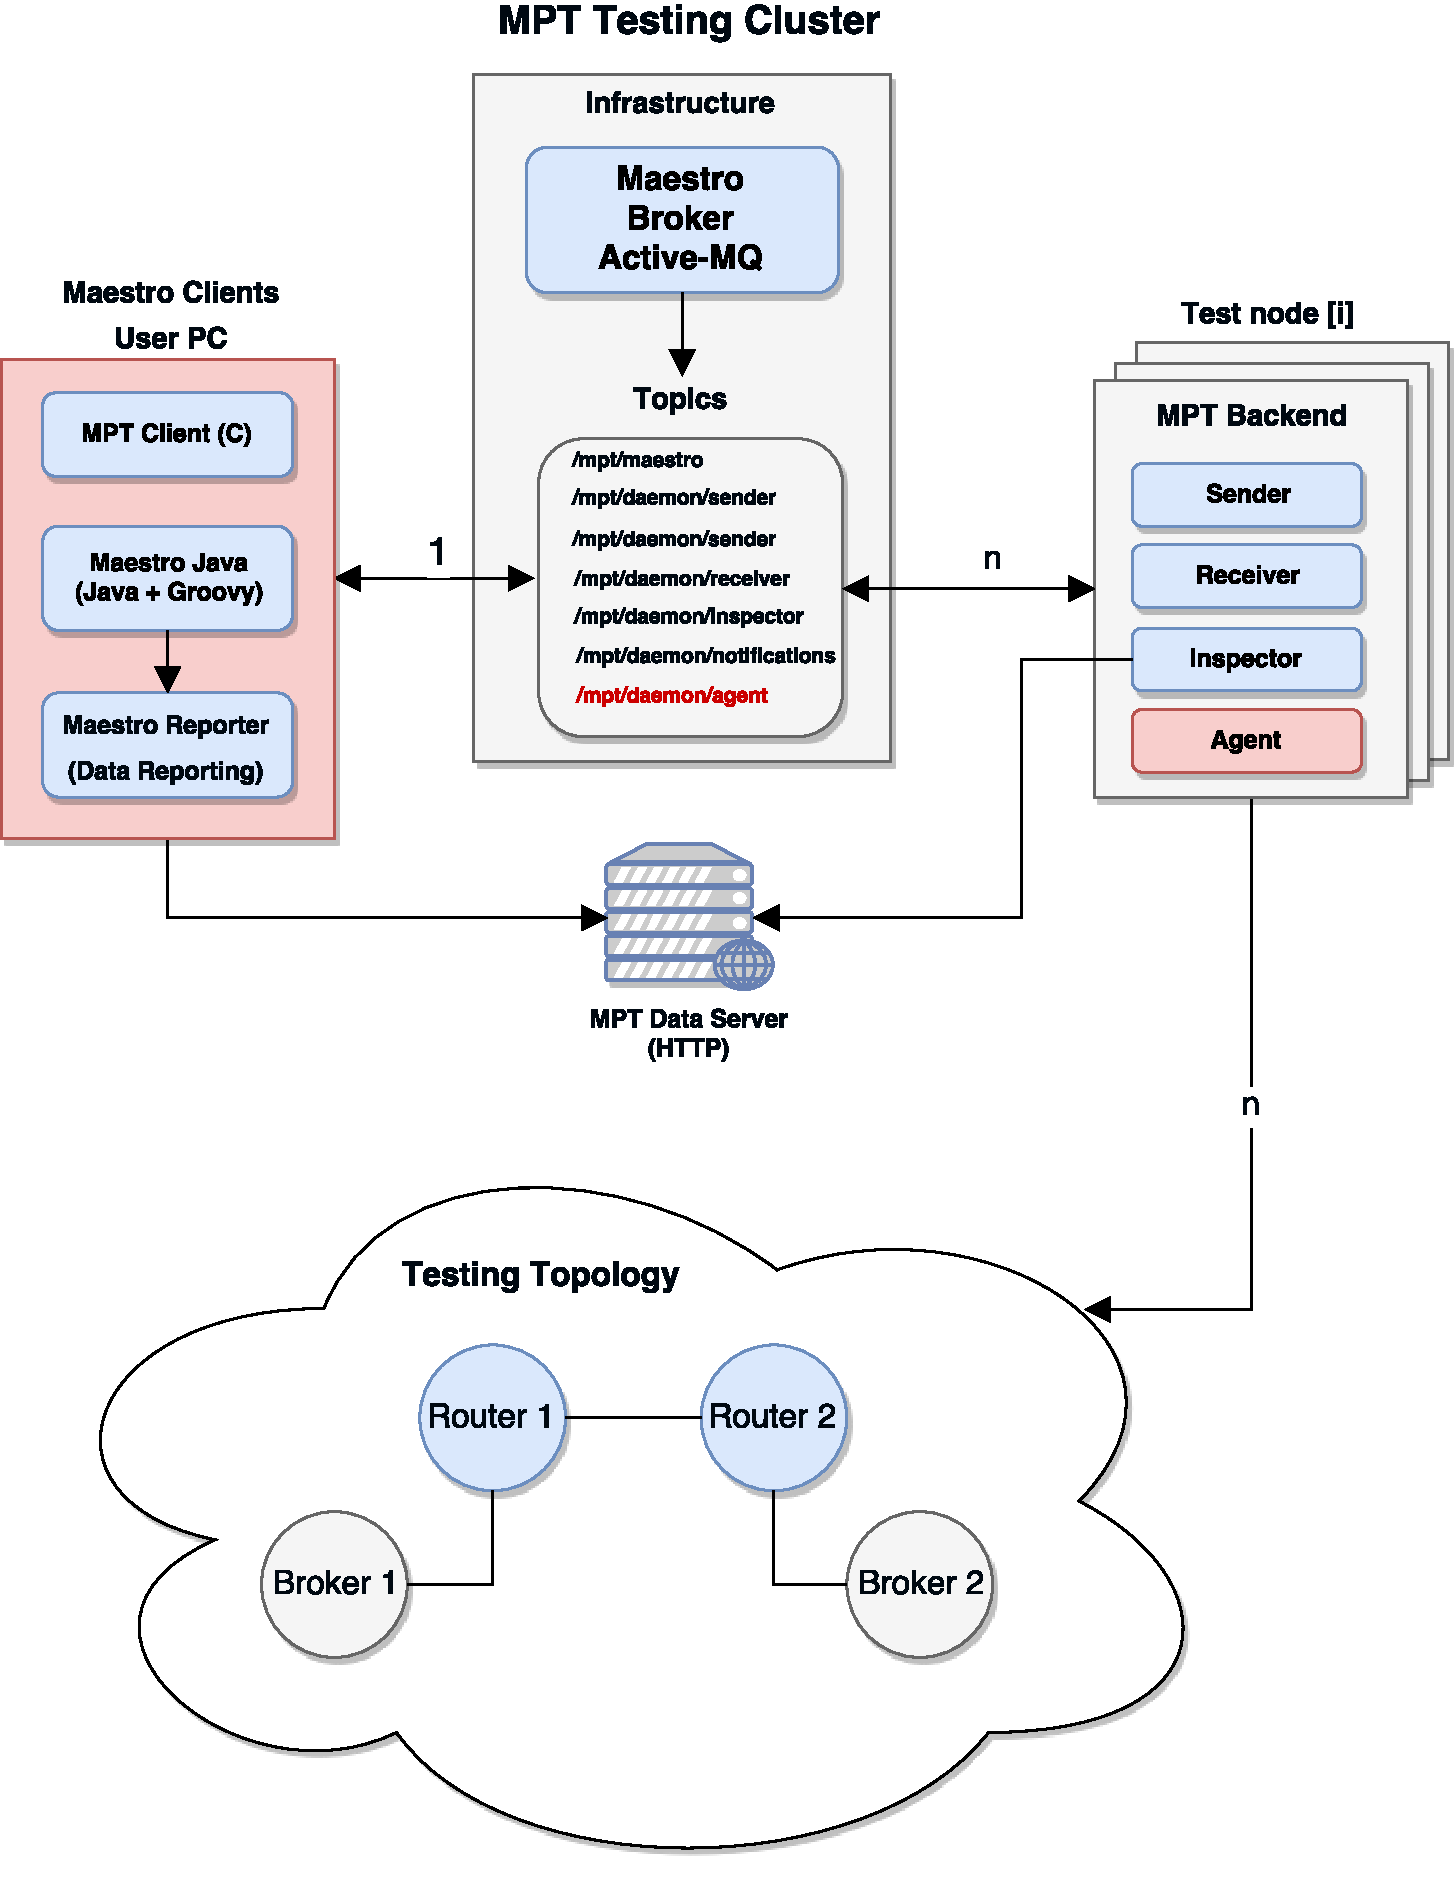
\includegraphics[width=15cm]{obrazky-figures/msg_perf_tool_for_router.pdf}
  \caption{Architecture of updated Maestro for testing of Qpid-dispatch router.}
  \label{fig:msg_perf_tool}
\end{figure}


\subsection{\todo{more subsections about module}}

\section{Performance and Testing Metrics of Qpid-Dispatch Performance Module}

\section{Collected Data Evaluation}

\chapter{Implementation}
\label{Implementation}

\section{Used Technologies}

\subsection{Ansible}

\subsection{Docker}
Using for testing Ansible roles (remove?)

\section{Topology Generator}

\subsection{Template Generator}

\subsection{Generation of Variables}

\subsection{Configuration Files Generation and Deployment}

\section{Qpid-Dispatch Performance Module}

\subsection{TODO - more subsections about implementation}

\chapter{Experimental Evaluation}
\label{Experimental Evaluation}

\section{Performance Testing on Various Generated Topology}

\section{Testing results}

\chapter{Future work and ideas}
\label{Future work and ideas}

\chapter{Summary}
\label{Conclusion}
%=========================================================================
